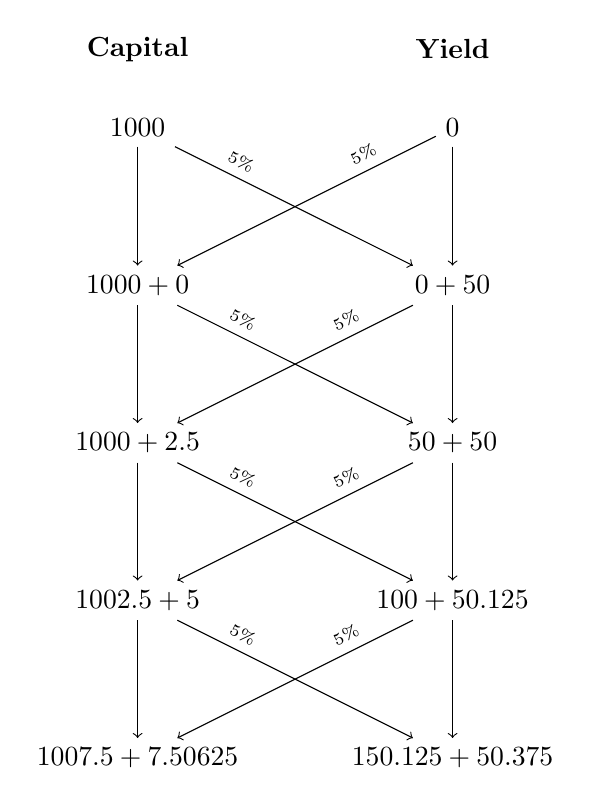
\begin{tikzpicture}
    \path (-2, 1)  node[fill=white, align=center]     {\textbf{Capital}};
    \path (2, 1)   node[fill=white, align=center]     {\textbf{Yield}};
    \path (-2, 0)  node[fill=white, align=center](x1) {1000};
    \path (2, 0)   node[fill=white, align=center](y1) {0};
    \path (-2, -2) node[fill=white, align=center](x2) {\(1000 + 0\)};
    \path (2, -2)  node[fill=white, align=center](y2) {\(0 + 50\)};
    \path (-2, -4) node[fill=white, align=center](x3) {\(1000 + 2.5\)};
    \path (2, -4)  node[fill=white, align=center](y3) {\(50 + 50\)};
    \path (-2, -6) node[fill=white, align=center](x4) {\(1002.5 + 5\)};
    \path (2, -6)  node[fill=white, align=center](y4) {\(100 + 50.125\)};
    \path (-2, -8) node[fill=white, align=center](x5) {\(1007.5 + 7.50625\)};
    \path (2, -8)  node[fill=white, align=center](y5) {\(150.125 + 50.375\)};
    
    \draw[->] (x1) -- (x2);
    \draw[->] (x2) -- (x3);
    \draw[->] (x3) -- (x4);
    \draw[->] (x4) -- (x5);
    
    \draw[->] (y1) -- (y2);
    \draw[->] (y2) -- (y3);
    \draw[->] (y3) -- (y4);
    \draw[->] (y4) -- (y5);
    
    \draw[->] (x1) -- node[near start, sloped, above] {\footnotesize{\(_{5\%}\)}} (y2);
    \draw[->] (x2) -- node[near start, sloped, above] {\footnotesize{\(_{5\%}\)}} (y3);
    \draw[->] (x3) -- node[near start, sloped, above] {\footnotesize{\(_{5\%}\)}} (y4);
    \draw[->] (x4) -- node[near start, sloped, above] {\footnotesize{\(_{5\%}\)}} (y5);
    \draw[->] (y1) -- node[near start, sloped, above] {\footnotesize{\(_{5\%}\)}} (x2);
    \draw[->] (y2) -- node[near start, sloped, above] {\footnotesize{\(_{5\%}\)}} (x3);
    \draw[->] (y3) -- node[near start, sloped, above] {\footnotesize{\(_{5\%}\)}} (x4);
    \draw[->] (y4) -- node[near start, sloped, above] {\footnotesize{\(_{5\%}\)}} (x5);
\end{tikzpicture}
